\documentclass[10.5pt]{article}
\usepackage{amsmath}
\usepackage{fancyhdr}

%删除线效果
\usepackage{ulem} 

\usepackage{amsthm}
\usepackage{scalerel} %调整积分符号大小
\usepackage{tikz}
\usepackage{bbold}
\usepackage{enumitem}
\usepackage{eqlist}

%背景色及边框

\usepackage{lipsum}
\usepackage{tcolorbox}

%调整积分符号大小
\def\stretchint#1{\vcenter{\hbox{\stretchto[400]{\displaystyle\int}{#1}}}}
\def\scaleint#1{\vcenter{\hbox{\scaleto[4ex]{\displaystyle\int}{#1}}}}





%M.C Paining 
\usepackage{tikz}
\usetikzlibrary{automata} 
\usetikzlibrary{positioning} 
\usetikzlibrary{arrows} 
\usepackage{enumitem}
\usepackage{pgfplots}
\tikzset{node distance=2.5cm,
      every state/.style={ semithick, fill=gray!10},
      initial text={},
      double distance=2pt,every edge/.style={draw,
      ->,>=stealth',auto,
semithick}}
\let\epsilon\varepsilon

\usepackage{bm}
\usepackage{mathrsfs}
\usepackage{undertilde}
\usepackage{xeCJK}
\usepackage{graphicx}
\setCJKmainfont{PingFangSC-Light}
\newcommand*\circled[1]{\tikz[baseline=(char.base)]{
            \node[shape=circle,draw,inner sep=2pt] (char) {#1};}}
\newcommand{\transmtx}[0]{\utilde{\mathcal{P}}}
\newcommand{\srv}[0]{\{X_n\}_{n \in \mathcal{N}}}
\newcommand{\prob}[0]{\mathcal{P}}
\newcommand{\hilight}[1]{\colorbox{orange!20}{#1}}
\newcommand{\vect}[2]{\overrightarrow{#1}_{#2}}
\newcommand{\expt}[0]{\mathbb{E}}



\usepackage{ amssymb }
\usepackage[utf8]{inputenc}
\usepackage[english]{babel}
\usepackage{color}
\usepackage{xcolor}
\usepackage[left=1in,top=1in,right=1in,foot=1in]{geometry}
\usepackage{graphicx}
\setCJKmainfont{Kai}
\newenvironment{changemargin}[2]{%
  \begin{list}{}{%
    \setlength{\topsep}{0pt}%
    \setlength{\leftmargin}{#1}%
    \setlength{\rightmargin}{#2}%
    \setlength{\listparindent}{\parindent}%
    \setlength{\itemindent}{\parindent}%
    \setlength{\parsep}{\parskip}%
  }%
  \item[]}{\end{list}}
\renewcommand{\arraystretch}{1.1}
\setlength\parindent{0in}
\pagestyle{fancy}

\fancyhf{}
\lhead{MATH\,303\,\,\, Stochastic process 随机过程}
\rhead{\scriptsize{\copyright \,Shihao Tong All Right Resvered}}
\rfoot{Page \thepage}
\renewcommand{\headrulewidth}{0.5pt}



\begin{document}

\theoremstyle{definition}
\newtheorem{definition}{Definition}

\theoremstyle{proposition}
\newtheorem{proposition}{Proposition}

\theoremstyle{lemma}
\newtheorem{lemma}{Lemma}

\theoremstyle{theorem}
\newtheorem{theorem}{Theorem}

\theoremstyle{collary}
\newtheorem{collary}{Collary}



%\begin{flushright}
%  % EDIT THIS NEXT LINE: Replace ``Name'' with your own name
%%   \large{\textbf{Shihao Tong (Owen)}}
%% \\
%  % EDIT THIS NEXT LINE: Replace ``12345678'' with your own student number
%%   \large{\textbf{38191201}}
%\end{flushright}

% Edit this line for title
%\large{\textbf{Stat 305 Statistical Inference}}

\def\stretchint#1{\vcenter{\hbox{\stretchto[400]{\displaystyle\int}{#1}}}}
\def\scaleint#1{\vcenter{\hbox{\scaleto[4ex]{\displaystyle\int}{#1}}}}
%
%\normalsize


%\begin{tabular*}{6.5in}{c}
%\hline
%\end{tabular*}
%
%\bigskip

\theoremstyle{remark}
\newtheorem{remark}{Remark}


\begin{changemargin}{-0.125in}{0in}


在随机过程中,将随机变量看做关于时间的变量,定义其所有可以取值的集合为\textit{State Space},简写为$\mathcal{S}$。且目前只讨论$\mathcal{S}$是有限或者是有限可数的情况。通常也可以将其结论推广至无限应用。

\bigskip

\begin{enumerate}
	
	\item \textbf{Discrete Time Markov Chain}
	
	\smallskip
	
	\begin{enumerate}
	
	\item \textbf{Basic Notations and Definition} 
	\begin{definition}(Markov Chain 马尔科夫链)\,\,\,\,\,
		Let $\{X_n\}_{n \in \mathcal{N}}$ be a series of r.v in $\mathcal{S}$. Then we say $\{X_n\}_{n \in \mathcal{N}}$ is a Markov Chain or has Markov properties if: $\forall\, n \in \mathcal{N}, \forall \, x_i \in \mathcal{S}$ 
		\[
		\mathcal{P}(X_{n+1} = x_{n+1} \, \, | \, \, X_n = x_n, \,X_{n-1} = x_{n-1}, \,...\, , X_0 = x_0) = \mathcal{P}(X_{n+1}\,\,|\,\, X_n = x_n)
		\]
	\end{definition}
	 This means the next behavior only depends on the current status and nothing to do with how it get here. For example, the random walk, your position next second depends only on where you are now. 
	 
	 \medskip
	 
	 注意以上的符号用法中,我们用$X_n$的下标$n$指代时刻$n$,即$t = n$时(假定时间是离散的)并假设无论在哪一个时刻在给定的\textit{state}下,都有固定的概率分布,该性质称之为\textit{time homogeneity}。数学定义为
	 
	 \smallskip
	 
	 
	 \begin{definition}(Time Homogeneity) We say a Markov chain is time homogeneity if 
	 \[
	 \forall \, (x,y)\,\in\,\mathcal{S}^2, \,\,\mathcal{P}(X_{n+1} = x\,|\, X_n = y)
	 \]
	 is all the same for all time $n$.	
	 \end{definition}
	 
	 
	 \smallskip
	 
      \begin{tcolorbox}[notitle,boxrule=0pt,colback=yellow!80,colframe=blue!20]
       Summary:Markov Chain 的两点非常强的假设
       \begin{itemize}
       	\item 下一时刻的状态只依赖于当前状态,与之前到达路径无关(Markvo Property)
       	\item 无论哪个时刻,两两状态间的概率不变(Time Homogeneity)
       \end{itemize}
       \end{tcolorbox}
   	 
	 \smallskip
	 
	 
	 对于概率通常用$\mathcal{P}_{ij}$表示,意为目前在$\textit{state} = X_n = i$状态下,下一步到$X_{n+1} = j$的概率。且由于是概率分布,有结论
	 \[
	 p_{ij} > 0,\,\,\,\,\sum^\infty_{j=0}\, p_{ij} = 1 
	 \]
	
     The second property can be proved \textcolor{red}{made up later}. Then consequently we can define the \textit{transition matrix} of M.C as the collection of all element $\mathcal{P}_{ij}$ as 
     \[
     (\utilde{\mathcal{P}})_{ij} = \mathcal{P}_{ij}  
     \]
     即矩阵的第$i$行$j$列个元素是从\textit{state} $i$ 到 \textit{state} $j$ 的概率。因此行向量各个元素和为1。注意\textit{transition matrix}一定是方阵。
     
     \medskip
     
     \begin{remark} \textit{Let the prob distribution of $X_n$ (at time $n$) is $\mu = (\mu_1, ..., \mu_N)$. Then the prob. distribution of $X_{n+1}$ is $\mu \cdot \utilde{\mathcal{P}}$ by definition of matrix product.}
     \end{remark}
     
     \medskip
     
     \begin{proof}
     	Now we are asking for $\mathcal{P}(X_{n+1} = s_j)$(Notice this is different form asking the M.C properties). First we have 
     	\[
     	\mathcal{P}(X_{n+1} = s_j) = \sum_{k \in \mathcal{S}}\, \mathcal{P}(X_{n+1} = s_j, \,X_n = s_k)
     	\]
     	this is because $\{X_n = s_k\}_{k \in \mathcal{S}}$ form a complete set of mutually exclusive event. Then by conditional probability we have 
     	\[
     	 = \sum_{k \in \mathcal{S}} \mathcal{P}(X_{n+1} = s_j\,| \,X_n = s_k) \mathcal{P}(X_n = s_k)
     	\] 
     	\[
     	 = \sum_{k \in \mathcal{S}} \mu_k \cdot (\utilde{\mathcal{P}})_{kj}
     	\]
     	which is exactly the matrix product.
     \end{proof}
     
     
     \medskip
     
     值得注意的是,这里的矩阵乘法是向量右乘矩阵,而非一般的左乘。最后一步的$\mu$的角标指的是第$k$个state。
     \medskip
     
     \begin{remark}(When State space is infinite) When $\mathcal{S}$ is not finite or countable, then we can generalize all concepts to infinite case. For example the transition matrix with infinite rows and column. 
     \end{remark}
     
     \medskip
     
     \begin{remark}
     	If we start with $X_0$ under an initial distribution $\mu = (\mu_1, \mu_2)$(consider two states case, \underline{$\mu$ is a prob distribution on $\mathcal{S}$}) with corresponding transition matrix $\utilde{\mathcal{P}}$. Then we have the prob. distribution of $X_n$ equals $\mu\cdot\transmtx^n$.
     \end{remark}
     
     \medskip
     
     \textcolor{red}{Does the initial prob distribution the same as a row in the transition matrix?} 
     
     \smallskip
     
     \medskip
     
     \textcolor{blue}{个人理解\circled{1}所谓\textit{initial distribution}是说目前整个随机过程还并未开始,该概率分布指的是在第一个时刻进入其中某个$state$的概率,与\textit{transition matrix}中元素代表的概率不同。\circled{2}无需纠结于Remark3。形式上看似$\mu \cdot \transmtx^n$并非只依赖于上一时刻的状态(因为至少有$\mu$在,看似依赖于初始分布)。其实所谓的只依赖于上一刻是指的上一个状态是$\mu \cdot \transmtx^{n-1}$,即需要上一时刻的概率分布必须是充分的。一直右乘同一个矩阵说明性质\textit{time homo.}。}
     
     \medskip
     
     \begin{definition}(Stationary Distribution) \,\,Let $\{X_n\}_{n \in \mathcal{N}}$ be a M.C with transition matrix $\transmtx$, and $\mu$ be a distribution on $\mathcal{S}$. We say that $\mu$ is a \textit{stationary distribution} if $\mu \cdot \transmtx = \mu$.
     \end{definition}

     \medskip
     
     \begin{proposition}\,\, If $\srv$ converges to a distribution $\mu$ as $n \rightarrow \infty$, then $\mu$ is stationary.
        \begin{proof}
        	Let $\mu_k$ be the prob. distribution of $X_k$. Then 
        	\[
        	\,u_{n+1} = \mu_n \cdot \transmtx \,\, \overset{n \rightarrow \infty}{\longrightarrow}\,\, \mu = \mu \cdot \transmtx
        	\]
        	Thus stationary.
        \end{proof} 
     \end{proposition}
       
    
       \begin{definition}\,\,(Graph Representation of a transition matrix) Using a \textit{directed graph} where each node represents a state and we draw arrow from $x$ to $y$ is $\mathcal{P}_{xy} > 0$, with weight $\mathcal{P}_{xy}$. This graph is called a \textit{transition diagram}.
       \end{definition}
       
       
       \smallskip
       
       \item \textbf{Chapman-Kolmogorov Equation}
       
       \medskip
       
       \begin{definition}(Generalized Remark3) For $n \in \mathcal{N}$, we define the \textit{n-step transition probability} as
       \[
       \mathcal{P}_{ij}^n = \mathcal{P}(X_{n} = j\,|\,X_0 = i)
       \]
       	and this consequently defines the \textit{n-step transition (prob.) matrix} $(\utilde{\mathcal{P}}^{(n)})_{ij} = \mathcal{P}_{ij}^n$(等式左边的$(n)$指的是\textit{step n},右边的$n$是指数).
       \end{definition}
       
       \smallskip
       
       \begin{remark}
       	\,\,\,One can also show (by induction on $n$ and appeal to time homo.) that 
        \[
        \forall \,\, k \in \mathcal{N},\,\,\,\mathcal{P}(X_{k+n} = j\,|\,X_k = i) = \mathcal{P}_{ij}^n
        \]
       \end{remark}
       
       \textcolor{red}{A attempt should be made later and make up here}
       
       \smallskip
       
       \begin{definition}(Chapman-Kolmogorov Equation)\,\,The Chapman-Kolmogorov Equation provides a method fpr solving the n-step probability. The equation is 
       \[
       \mathcal{P}^{n+m}_{ij} = \sum_{k = 0}^\infty \,\,\mathcal{P}_{ik}^n\cdot\mathcal{P}_{kj}^m
       \] 
       \end{definition}
       
       Interpretation of this equation is, starting from state $i$ and go through state $k$ at $t=n$ on the way to state $j$ where finally land at $t = m + n$.
       
       \begin{proof}
       \[
       	\mathcal{P}_{ij}^{n + m} = \mathcal{P}(X_{n+m} = j\,|\,X_0 = o)
       	\]
       	\[
       	= \sum_{k = 0}^\infty\mathcal{P}(X_{n+m} = j, \,X_n = k\,|\,X_0 = i)
       	\]
       	this is simply the total probability in case of conditional probability. Then 
       	\[
       	  = \sum_{k = 0}^\infty \mathcal{P}(X_{n+m} = j\,| X_n = k, X_0 = i) \cdot \mathcal{P}(X_n = k\,|\,X_0=i)
       	\]
       	this is achieved by
       	\[
       	\prob(A \cap B \,|\,C) = \frac{\prob (A\cap B\cap C)}{\prob(C)} = \frac{\prob(A\,|\,B\cap C)\prob(B\cap C)}{\prob(C)} = \prob(A\,|\,B\cap C)\cdot \prob(B \,|\,C)
       	\]
       	then by the definition of step transition we have 
       	\[
        = \sum_{k = 0}^\infty \,\,\mathcal{P}_{ik}^n\cdot\mathcal{P}_{kj}^m
       	\]
       \end{proof}
       
       \item \textbf{Classification of States(4.3 Ross)}
       
       \smallskip
       
       
       \begin{itemize}
       	\item (Accessibility) A state is \textit{accessible} from state $i$ if $\mathcal{P}_{ij}^n > 0$ for some $n \geq 0$.
        \item (Community) Two sates $i$ and $j$ are \textit{communicate} (i $\leftrightarrow$ j) if $i$ is accessible form $j$ and $j$ is accessible from $ii$. 
       \end{itemize}
       
       Above properties are can easily be checked by transition diagram. Communication is an \hilight{\textit{equivalence}} relation which satisfies \textit{reflexivity, symmetric and transitivity}. Reflexivity and symmetric are trivial by definition. Here prove transitivity. 
       
       \begin{proof}\,\, (Transitivity) Want to prove: if $i \leftrightarrow j$ and $j \leftrightarrow k$, then $i \leftrightarrow k$. The given condition can be interpreted as 
       \[
       \exists \,\, m \,\,\,\,s.t \,\, \prob_{ij}^m > 0,\,\,\, \exists\,\, n \,\,\,\,s.t. \,\, \prob_{jk}^n > 0
       \]
       	then by Chap.-Kolm. Equation we have 
       	\[
       	\prob_{ik}^{m + n} = \sum^\infty_{\rho}\,\prob_{i\rho}^m \cdot \prob_{\rho k}^n \geq \prob_{ij}^m\cdot \prob_{jk}^n > 0
       	\]
       	the $\geq$ is because the sum must include the case $\rho = j$, that is $j$ is just one case in the summation. \textcolor{blue}{Vice versa need to show $k$ can achieve $i$ in the same way.} 
       \end{proof}
       Therefore we can \hilight{partition} the space state into \textit{communicating class}. 
       
       \medskip
       
       \begin{definition} \,\,\,\,\,(Irreducibility) A M.C is said to be \textit{irreducible} if there is only one communicating class (e.g all states communicates with each other).
       \end{definition}
       
       For example the one dimensional random walk. 
        
       \medskip
       
       \medskip
       
       
      \begin{center}
      	
       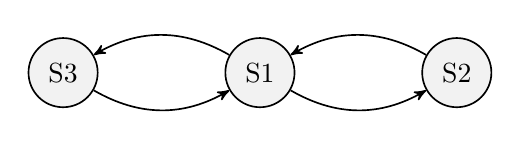
\begin{tikzpicture}
          \node[state] (s1) {S1};
          \node[state, right of=s1] (s2) {S2};
          \node[state, left of=s1] (s3) {S3};
          \draw (s1) edge[bend right]  (s2);
          \draw (s2) edge[bend right]  (s1);
           \draw (s3) edge[bend right]  (s1);
          \draw (s1) edge[bend right]  (s3);
       \end{tikzpicture}
        
       \end{center}
       
       \medskip
       
       
       \begin{definition}(Period) \,\,\,The state $i$ has \textit{period d} if $\mathcal{P}_{ii}^n = 0$ whenever $n$ is not divisible by $d$, and $d$ is the biggest integer with this property. If $d=1$ then, $i$ is called \textit{aperiodic}. Formally the definition is 
       \[
       p = gcd\{n : \mathcal{P}(X_n = i) \,|\, X_0 = i\}
       \]
       where \textit{gcd} is the greatest common divisor. Or another more understandable interpretation is: \textit{The period of a state i is the greatest common denominator (gcd) of all integers n > 0, for which $\mathcal{P}_{ii}^n>0$}.
       \end{definition}
       
       \medskip
       
       Notice the \textit{"period"} usually referred to a particular state. Each state may have different period. 
       
       \medskip
       
       \begin{proposition}\,\,\,If $i$ has period $d$ and $i \leftrightarrow j$, then $j$ also has period $d$.
           \begin{proof}\,\,\,\, By community we have 
           \[
           \exists \,\, n ,\, m \geq 0\,\,s.t. \,\,\,\prob_{ij}^n >0 \,\&\,\prob_{ji}^m > 0
           \]
       	   Since $i$ has period $d$, so we have, $\forall\,k$ s.t. $\prob_{jj}^k > 0$, we have
       	   \[
       	   \prob_{ii}^{m+n} \geq \prob_{ij}^n \prob_{ji}^m > 0\,\, \implies \,\, d \,|\, m+n
       	   \]
       	   \[
       	   \prob_{ii}^{m+n+k} \geq \prob_{ij}^n \prob_{jj}^k \prob_{ji}^m > 0\,\, \implies \,\, d \,|\, m+n+k
       	   \]
       	   both from C-K-E. The $|$ means devisable by (e.g $d \,|\, m+n$ means $(m+n)/d$ $\in \mathcal{Z}$). Then we have 
       	   \[
       	   \textcolor{red}{d \, |\, k \,\,\, \implies \,\,\,d \leq d'}
       	   \]
       	   where $d'$ is the period of $j$. By symmetric we can show $d' \leq d$ so pushing $d' = d$.
           \end{proof}
           The consequence of the proposition is that the periodicity is a class property (i.e all states in the same class has this property). 
       \end{proposition}
       
       \begin{definition} \,\,(Recurrence and Transience)\, Let $f_i = \prob(X_n = i\,\, \text{for some} \,\,n \geq 1\,|\,X_0 = i)$. We say $i$ is \textit{recurrent} if $f_i = 1$, and $i$ is \textit{transient} if $f_i < 1$.
       \end{definition}
       
       \medskip
       
       \hilight{注意$f_i$的定义:必须从零时刻时,从该state开始}.
       
       \medskip
       
       This definition measure the ability of a M.C to revisit a state. Another good property is, the state is either transient or recurrence, so we can split the state space into recurrent and transient spaces. 
       
       \medskip
       
       \begin{remark} If $\prob_{ii} = 1$ and $i$ is recurrent, then $i$ is called a absorbing state.
       \end{remark}
       
       \medskip
       
       The absorbing state $i$ usually looks like 
       
       \begin{center}
      	
       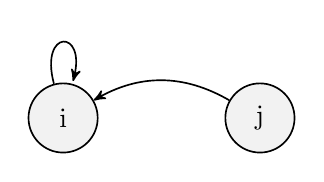
\begin{tikzpicture}
          \node[state] (i) {i};
          \node[state, right of=i] (j) {j};
          
          \draw (j) edge[bend right]  (i);
          \draw (i) edge[loop above]  (i);
       \end{tikzpicture}
        
       \end{center}
       
       注意定义中$\prob_{ii} = 1$ 意思是下一步只能到自己。
       
       \medskip
       
       \item \textbf{Properties of Recurrence and Transience}
       
       \medskip
       
       We first define the random variable $\mathcal{N}_i$ as
       \[
       \mathcal{N}_i = \# \{X_n = i\,|\, n \geq 0\}
       \]
       and it has a range $\mathcal{N} \, \cup \, \infty$. It can also be represented as 
       \[
       \mathcal{N}_i = \sum_{n = 0}^\infty \mathbb{1}_{(X_n = i)}
       \]
       简而言之,是一个计数过程。随机过程不断进行,每当其中一个时刻$X_k =i $,$\mathcal{N}_i$就加一。且$\mathcal{N}_i$ 的和中要求$n =0$ 开始, 暗指了必须从时刻0开始计数。where $\mathbb{1}_{(X_n = i)}$ is 1 if $X_n = i$ or 0 if $X_n \neq i$, just like a counting process or accumulator. Also if we think of $\mathbb{1}_{(X_n = i)}$ as a random variable, it follows a \textit{Bernoulli distribution} (either is or not). So 
       \[
       \mathbb{E}(\mathbb{1}_{(X_n = i)}) = 1 \cdot \prob(X_n = i) + 0 \cdot \prob(X_n \neq i) = \prob(X_n = i)
       \] 
       注意,上式的期望值当$n$取之不同时也不相同。
       
       \medskip
       
       \begin{proposition}
       	 \begin{itemize}
       	 
       	 	\item If $i$ is recurrent, then $\prob(\mathcal{N}_i = \infty\,|\,X_0=i) = 1$
       	 	
       	 	\medskip
       	 	
       	 	\item If $i$ is transient and $X_0 = i$, then $\mathcal{N}_i \sim$ \textit{Geom(1 - $f_i$)}. $(i.e,\prob(\mathcal{N}_i = m) = f_i^{m-1}(1 - f_i)), \mathbb{E}(\mathcal{N}_i) = 1/(1 - f_i)$.
       	 \end{itemize}
       \end{proposition}
       
       
       \medskip
       
       Interpretation of above proposition is, a recurrent sate is revisited $\infty$ many times, while for a transient state, then chain doesn't revisit the state after a certain times (and the probability to revisit is $f_i$). \textcolor{red}{proof made up later Jan 13th.}
       
       
       \medskip
       
       \begin{remark}
       	 \begin{itemize}
       	 	\item If state $i$ is recurrent, then $\mathbb{E}(\mathcal{N}_i \,|\, X_0 = i) = \infty$ (if transient, $\mathbb{E}$ < $\infty$).
       	 	\item If state space is finite, then some state must be recurrent. 
       	 \end{itemize}
       \end{remark}
       
       \medskip
       
       The first one is trivial \textcolor{blue}{may have some formal proof here}. The proof for second one is ---- we assume all states are transients, so there is no state visited after a certain time, so contradicted.
       
       \medskip
       
       Now we use \textit{n-step transition probability} to characterize recurrence and transience. 
       
       \begin{proposition}
       	We say state $i$ is recurrent if 
       	\[
       	\sum^\infty_{n=0}\,\prob_{ii}^n = \infty
       	\]
       	is transient if 
       	\[
       	 \sum^\infty_{n=0}\,\prob_{ii}^n < \infty 
       	\]
       \end{proposition}
       
       Less than $\infty$ means the probability is a concrete number (finite). 
       
       \begin{proof}
       	Only need to prove the expectation is the sum of n-step transition matrix. 
       	\[
       	\mathbb{E}[\mathcal{N}_i\,|\,X_0 = i] = \,\mathbb{E}[\sum^\infty_{n=0}\, \mathbb{1}_{(X_n = i)}\,|\,X_0 =i]
       	\]
       	\[ 
       	= \sum^\infty_{n=0} \mathbb{E} [\mathbb{1}_{(X_n = i)}\,|\,X_0 = i] = \sum^\infty_{n=0} \prob_{ii}^n
       	\]
       \end{proof}
       
       \begin{collary}
       	 If $i$ is recurrent and $i \leftrightarrow j$, then $j$ is also recurrent 
       \end{collary}
       
       \begin{proof}
       	The recurrent here is used to be integrated into the C.K.E. By comm. and rec. we have $\exists\,k, \,m$ s.t. $\prob_{ij}^k > 0$, $\prob_{ji}^m > 0$. Then $\forall\,n>0$ we have 
       	\[
       	\prob_{jj}^{m + n + k} = \sum_{s,t}\, \prob_{js}^m \prob_{st}^n\prob_{tj}^k \geq \prob_{ji}^m \prob_{ii}^n\prob_{ij}^k
       	\]
       	then we check the characterized recurrent definition
       	\[
       	\sum^\infty_{N = 0}\,\prob_{jj}^N \geq \sum^\infty_{n = 0}\,\prob_{jj}^{m+ n + k} \geq \sum^\infty_{n = 0} \prob_{ji}^m \prob_{ii}^n\prob_{ij}^k \geq \prob_{ji}^m (\sum^\infty_{n = 0} \prob_{ii}^n ) \prob{ij}^k = \infty
       	\]
       the first inequity is because the LHS start from $0$ while the RHS start actually from $m + k$. Then middle term of the the last term is infinity by recurrence of $i$. So we finally generate that the sum is infinity and thus $j$ is recurrent.
       \end{proof}
       
       So our consequence are 
       
       \begin{itemize}
       	\item Recurrence and transience are \hilight{class properties} (all states in the communicating class are all either transient or recurrent).
        
        \item The collory can be relaxed as "$i$ is recurrent and $i \rightarrow j$"
        \item If $i \rightarrow j$ but $j \nrightarrow i$, then $i$ is transient
        \end{itemize}
      \end{enumerate}
      
      
      \medskip
    
    \item \textbf{Model: Gambler's Ruin}
    
    \medskip
    
    The scenario is: a gambler has \$$n$ initially (capital) and play a game with probability $\bar{p}$ of winning \$1 and $1 - \bar{p}$ of losing \$1 otherwise. The gambler plays until he reach a goal of having \$$N$ $\geq$ $n$, and clearly his wealth follows a Markov Chain. 
    
    
    \medskip
    
    The transition diagram is one dimensional with $N + 1$ states (n $\in [0,N]$). The corresponding transition matrix is 
    \[
    \transmtx \, = \,
    \left(\begin{array}{ccccccc}
      1 & 0 &0 & ... & 0 & 0 & 0\\ 
      1-p & 0 & p & ... & 0 & 0 & 0\\
      0 & 1-p & 0 & p & ... & & 0\\
      0  & 0 &1-p & 0 & p & ... & 0\\  
      ... & ... &... &... &... &... & ...\\ 
      0 & 0 &... &... &0 &0 & 1\\    
      \end{array}\right)
    \]
    Obviously there are three communicating classes: $\{0\}$, $\{N\}$ and $\{1, ..., N-1\}$, where the fist two are aperiodic and the last class is of period 2. Then a reasonable question is, let $R$ be the event that the "gambler goes broke", and asking for $\prob(R \,|\, X_0 = n)$. 
    
    \medskip
    
    \underline{\textbf{Model:}}\,\, Now let $\prob(n) = \prob(R \,|\, X_0 = n)$. Then the boundary conditions are $\prob(0) = 1$ and $\prob(N) = 0$. Then for $1 \leq n \leq  N-1$ we have 
    \[
    \prob(\mu) = \prob(R \,|\, X_0 = \mu) = \prob(R\,|\,X_1 = \mu+1)\prob(X_1 = \mu+1\,|\,X_0 = \mu) 
    \]
    \[
    \,\,\,\,\,\,\,\,\,\,\,\,\,\,\,\, \,\,\,\,\,\,\,\,\,\,\,\,\,\,\,\, \,\,\,\,\,\,\,\,\,\,\,\,\,\,\,\, \,\,\,\,\,\,\,\,\,\,\,\,\,\,\,\,+ \prob(R\,|\,X_1 = \mu -1)\prob(X_1 = n-1\,|\,X_0 = \mu) 
    \]
%    \textcolor{blue}{The relationship is given by the difference equation (no typo here, not differential.)} 
     
    This can be generated by conditioning on $R \,\cap\, X_0 = \mu + 1$ and $\mu - 1$Then we have 
    \[
    \prob(\mu) = \prob(\mu+1)\cdot \bar{p} + \prob(\mu-1)\cdot (1 - \bar{p})
    \]
    which is a 2nd order linear recurrence. Consider the Characteristic equation in $x$, we have 
    \[
    x = x^2 \cdot \bar{p} + 1 \cdot (1 - \bar{p}) \implies \bar{p}x^2 -x + (1 - \bar{p}) = 0
    \]
    check $\Delta = (2 \bar{p} - 1)^2 \geq 0$. So two cases are 
    
    \medskip
    
    \begin{itemize}
    	\item $\Delta > 0 \equiv \bar{p} \neq 1/2$ : Two roots are $x_1 = 1$ and $x_2 = (1 - \bar{p})/\bar{p} = a$ (a for short). Then the 'general solution' is 
    	 \[
    	 x = \prob(n) = \alpha\cdot x_1^n + \beta \cdot x_2^n
    	 \]
    	 where $\alpha\,\&\,\beta$ need to be determined by the boundary conditions. Plugging in the boundary condition 
    	 \[
    	 \alpha = \frac{a^N}{1 - a^N},\,\,\beta = \frac{1}{1 - a^N}
    	 \]
    	 so the general solution is 
    	 \[
    	 \prob(n) = \frac{a^N - a^n}{a^N - 1} = 1 - \frac{a^n - 1}{a^N -1}
    	 \]
    	 \item $\Delta = 0 \equiv \bar{p} = 1/2$: Similar to case in differential equation, when encounter with repeated root, we assume the general solution to be 
    	 \[
    	 \prob(n) = \alpha \cdot x^n + \beta\cdot n x^n
    	 \]
    	 and using the boundary condition solving for coefficients. We get 
    	 \[
    	 \prob(n) = 1 - \frac{n}{N}
    	 \]
    	 
    \end{itemize}
    So in summary, the solution is 
      \begin{equation}
      	\prob(n) = \begin{cases}
      		       1 - \frac{a^n - 1}{a^N -1}, \text{if}\ \bar{p} \neq \frac{1}{2}\\
      		         1 - \frac{n}{N}, \text{if}\ \bar{p} = \frac{1}{2}
      	           \end{cases}
      \end{equation}
      
      \begin{remark}
      	This type of problem is typically interpreted as a one dimensional random walk with absorbing boundaries. 
      \end{remark}
      
      \medskip
      
      \item \textbf{Model: Random walk in $\mathcal{Z}^1$}
      
      \medskip
      
      We consider the (discrete) uniform random walk and questioning is the state recurrent or transient? 
      
      \medskip
      
      \textbf{Solution:} First we will need a tool called \textit{Stirling's formula}, which is a approximation of $n!$. That is 
      \[
      n! \,\, \approx \,\,\sqrt{2\pi n}\,\,\big(\frac{n}{e}\big)^n
      \]
      As we showed previously, the way to prove transience or recurrence is by showing the sum of all n-step transition probability is $\infty$ or not. Let's consider the 1 dimensional case starting form 0. Since the recurrence and transience are class properties, so it is valid to just show 0 is feasible. 
      
      \medskip
      
      Starting form 0. If we want to come back to 0, we must take $2n$ steps (since one dimensional) and easy to see $\prob_{00}^{2n+1} = 0$. Thus 
      \[
      \prob_{00}^{2n} = \bigg(\frac{1}{2}\bigg)^n \cdot \,\binom{2n}{n} = \frac{\binom{2n}{n}}{2^{2n}}
      \]
      which means, we have to move $2n$ steps in total and want $n$ to be forward and $n$ to be backwards to get back to 0. The summation becomes 
      \[
      \sum_{n = 0}^\infty\,\prob^n_{00} = \sum_{n = 0}^\infty\,\frac{\binom{2n}{n}}{2^{2n}} = \sum_{n = 0}^\infty\, \frac{(2n)!}{(n!)^2\cdot 2^{2n}}
      \]
      apply the stirling's formula to replace the factorial, we get 
      \[
      \sum_{n = 0}^\infty\, \frac{1}{\sqrt{\pi n}} \rightarrow \infty
      \]
      we can compare to the series $1/n$ (we know $1/n$ is divergent and $1/\sqrt{n}$ is greater than it), so the series diverges and therefore the \hilight{symmetric 1-dimension random walk is recurrent.} \textcolor{blue}{Also we can show that the asymmetric 1-dimension random walk is transient.}
      
      \medskip
      
      \item \textbf{Model: Random walk in $\mathcal{Z}^d$}
      
      \smallskip
       
      By means of \textit{Characteristic function}. Notations: we define $\overrightarrow{e}_j's$ are the canonical basis of $\mathcal{Z}^d$. So we define the R.W at steps $\overrightarrow{X}_i$ with probability 
      \[
      \prob(\overrightarrow{X}_i = \overrightarrow{e}_j) =       \prob(\overrightarrow{X}_i = -\overrightarrow{e}_j) = \frac{1}{2d}
      \]
      通俗讲,在第$i$步时,向$\overrightarrow{e}_j$方向走的概率为1/2d(2d是因为有d个维度,则有2d个方向)。Then let $\overrightarrow{S}_0 = \overrightarrow{0}$ and $\overrightarrow{S}_n = \text{position after n steps} = \sum_{i=1}^n\overrightarrow{X}_i$, then 
      \[
      \overrightarrow{S}_{n+1} = \overrightarrow{S}_n + \overrightarrow{X}_{n+1}
      \]
      then we can define the transition probability as 
      \[
      \prob(\vect{S}{n+1} = \vect{S}{} \pm \vect{e}{j}\,|\,\vect{S}{n} = \vect{S}{}) = \frac{1}{2d}
      \]
      
      \begin{definition}
      	For $\vect{k}{} \in \mathcal{R}^d = (k_1, ..., k_d)$, we can define $\phi(\vect{k}{})$, that is the characteristic function of $\vect{S}{n}$ evaluated at $\vect{k}{}$,s.t
      	\[
      	\phi_n(\vect{k}{}) = \mathbb{E}(e^{i\vect{k}{} \cdot \vect{S}{n}})
      	\]
      \end{definition}
      
      \begin{remark}
      	\begin{itemize}
      		\item The product of $\vect{k}{}$ and $\vect{S}{n}$ is scalar product in $\mathcal{R}^d$ of $\vect{k}{}$ and $\vect{S}{n}$. So 
      		      \[
      		      \vect{k}{} \cdot \vect{S}{n} = \sum^n_{i=1}\vect{k}{}\cdot \vect{X}{i}
       		      \]
       		\item The Euler's formula can be applied here 
       		      \[
       		      e^{i\theta} = \cos\theta + i \sin\theta
       		      \]
      	\end{itemize}
      \end{remark}
      
      
      \begin{theorem}
      	The symmetric R.W in $\mathcal{Z}^d$ is \textit{recurrent} if $d = 1,2$ and is \textit{transient} if $d \geq 3$. 
      \end{theorem}
      
      \begin{proof}
      	\textcolor{blue}{make up later Jan 22nd}
      \end{proof}
      
      
      
      \item \textbf{Limiting probability}
      
      \smallskip
      
      The limiting probability is simply the proba. distribution of being at sate $i$ as $n$ goes to infinity which is 
      \[
      \pi_j = \lim_{n \rightarrow \infty} \mathcal{P}(X_n = j\,|\, X_0 = i)
      \]
      this also accounts for the \textit{proportion of time the M.C stays in each state in the long run}. Let $m_i$ be the \textit{mean \# of transaction returning to i, starting from i}. Then we have the proposition that the \hilight{proportion of time that the M.C stay at i must equal to 1/$m_i$ in the long run, so $\pi_i$ =1/$m_i$.} Also notice, the limiting distribution depends does not depends on the initial state, so we can also write is as 
      \[
      \pi_j = \lim_{n \rightarrow \infty} \prob(X_n = j),\,\,\forall \,  
      \]
      
      \begin{proof}
      	\textcolor{blue}{text book chapter 4 P216. incredible }
      \end{proof}
      
      \begin{definition}
    		A state $i$ is said to be positive recurrent if $m_i < \infty$; it is said to be null recurrent if $m_i = \infty$
    	\end{definition}
    	
    	It is easy to check that the one dimension symmetric random walk is null recurrent by 
    	\[
    	m_i = \sum_{n} 2n \cdot P(T = 2n) = \sum_{n} \frac{1}{\sqrt{\pi n}} = \infty
    	\]
        Notice that: \circled{1} Positive and null recurrence are both class properties \circled{2} If the state space is finite, then all recurrent states are positive recurrent. 
        
        \begin{definition}
        	An aperiodic positive recurrent state is called \textit{ergodic}. A ergodic M.C is a M.C whose states are all ergodic.
        \end{definition}
      
        \begin{theorem}
        For an irreducible ergodic M.C, $\pi_{j} = \lim_{n\rightarrow \infty} \prob_{ij}^n$ always exists for all $j$, independent of $i$.
        \end{theorem}

        In addition: \circled{1} $\underline{\pi}$ is the unique solution to 
        \[
        \underline{\pi} \cdot \transmtx = \underline{\pi}\,\,\,\,\&\,\,\,\sum_{j \in \mathcal{S}}\pi_j = 1
        \]
         \circled{2} $\pi_j = 1/m_j$, where $m_j$ is the mean return time to $j$ ($\pi_i>0$). \circled{3} $\pi_j$ by its definition can be written as 
         \[
         \pi_j = \lim_{n\rightarrow \infty} \frac{\# \text{visits to $j$ by total $n$ transition}}{n} = \text{long run proportion of time spent at $j$}
         \]        
      
        注意,对于\circled{1}来说,如果想用不等式解出distribution,那么需要check前提条件:\hilight{irreducible and positive re-} \hilight{-current.} 其实对于大部分情况来说很好检查:irreducible 只需要看是否只有一个communicating class (直接检查是否transition matrix没有0在其中);对于positive recurrent来说,往往遇到的情况都是finite 的 state space,根据之前的结论可知,recurrent state必然是positive recurrent。
        
        \begin{definition} (Probability for inverse M.C) Assume the M.C has been operating for a long time with stationary distribution $\pi$ \textcolor{red}{the limiting probability?}. Let $Y_n = X_{N-n}$, take $N$ as the time that M.C has already operated. Then we define the time inverse transition probability for $Y_n$ as
        \[
        \mathcal{Q}_{ij} = \prob(Y_n = j\,|\,Y_{n-1} = i) = \frac{\pi_j \prob_{ji}}{\pi_{i}}
        \]	
        \end{definition}
       
       \begin{proof}
       	\textcolor{blue}{$Y_n$ is also a M.C Notes on Jan.31}
       \end{proof}
       由于$Y_n$是从$X$的序列tracing back, 所以证明时注意站在$X$的视角注意角标。Notice the existence of stationary distribution is necessary for the inverse M.C to be homogeneous. 
       
       \begin{definition}
       	We say the M.C is time reversible if 
       	\[
       	\mathcal{Q}_{ij} = \mathcal{P}_{ij}
       	\]
       \end{definition}
       
       \begin{remark}
       	 \begin{itemize}
       	 	\item
         	 We always have $P_{ii} = Q_{ii}$
         	 \item For a reversible M.C 
         	 \[
         	 \pi_i \prob_{ij} =\pi_j \prob_{ji}
         	 \]
         	 which is interpreted as the \textit{fraction of jumps at stationarity.} This forms a so-called \textit{detailed balance.}
         \end{itemize}
       \end{remark}
       
       \begin{proposition}
       	Let $X_n$ be a \hilight{ergodic irreducible} M.C. If we can find a series of $x_i \geq 0$, s.t $x_i \prob_{ij} = x_j \prob_{ji}$ and $\sum x_i = 1$, then $x_i = \pi_i$ and M.C is time reversible.
       \end{proposition}
       
       \begin{proposition}
       	(Kolmogorov's criteria): An ergodic MC is time reversible \textbf{iff} for $\forall$ finite sequence of states $(i_1, i_2,...,i_n)$, we have 
       	\[
        \prob_{i_1i_2} \prob_{i_2i_3}... \prob_{i_ni_1} =  \prob_{i_1i_n}  \prob_{i_ni_{n-1}}... \prob_{i_2i_1}
       	\]
       	visualization is 
       	\begin{center}
      	
       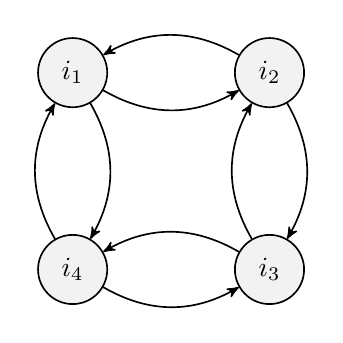
\begin{tikzpicture}
          \node[state] (i) {$i_1$};
          \node[state, right of=i] (j) {$i_2$};
          \node[state, below of=j] (k) {$i_3$};
          \node[state, left of=k]  (l)  {$i_4$};
          
          \draw (j) edge[bend right]  (i);
          \draw (i) edge[bend right]  (j);
          \draw (j) edge[bend left]  (k);
          \draw (k) edge[bend left]  (j);
          \draw (k) edge[bend right]  (l);
          \draw (l) edge[bend right]  (k);
          \draw (l) edge[bend left]  (i);
          \draw (i) edge[bend left]  (l);
       \end{tikzpicture}
       \end{center}
       \end{proposition}
       
       \textcolor{red}{prove Feb 3rd} starting from the stationary distribuion. 
       
       \medskip
       
       \underline{\textbf{Example: Ehrenfest Chain}}
       
       \smallskip
       
       有两个罐子,一共M个球。每一步随机从其中一个罐子中拿一个球放到另一个罐子中。Let $\mathcal{S} = \{0,1,...,M\}$ and $X_n$ be the \# of balls in urn 1. The probability is defined as 
       \[
       \prob_{01} = 1\,\,\,\,\prob_{M,M-1} = 1\,\,\,\,\prob_{i, i+1} = \frac{M - i}{M}\,\,\,\,\prob_{i, i-1} = \frac{i}{M}
       \]
      
        The chain is ergodic. The stationary distribution can be found by either solving the detailed balance equation or guess and check. The result turn out to be a binomial distribution of $\pi$
        \[
        \pi \,\,\sim \,\, Bino(M, \frac{1}{2})
        \]
        
        \medskip
        
        \item \textbf{Barnching Process}
        
        \smallskip
        
        \begin{definition} \,(Branching Process) Let $Z_i$ be the \# of individuals at generation $i$, $y_{n,i}$ be the \# of offsprings of $i$ th individual at generation $n$. Then the \textit{branching process} is defined as the sequence of r.v. $\{Z_n\}_{n \geq 0}$ such that 
        \begin{equation}
      	           \begin{cases}
      		       Z_0 = 1\\
      		       Z_{n+1} = \sum^{Z_n}_{i = 1}\,y_{n, i}\\ 
      	           \end{cases}
      \end{equation}
            This is called the reproduction law. 
        \end{definition}
        
        
             	\begin{itemize}
             	
        		\item $Z_n$ defines a discrete time M.C on $\mathcal{N}$.
        		\item  $\{0\}$ defines a absorbing $\rightarrow$ recurrent class. We assume the probability $\prob(y_{n,i}= 0) > 0 $ and 0 is accessible form all other states, so all other states are transient.
        		\item Since the finite set of transient states can only be visited finite times. So we can expect, in the long run, $Z_n$ is either $\infty$ or 0 as $n\rightarrow\infty$.
        	\end{itemize}
        	
        	\medskip
        
            \begin{definition} (Probability Generation Function) Let $X$ be a r.v on $\mathcal{N}$. Then the probability generating function of $X$ is 
            \[
            G_X(s) = \mathbb{E}_X(s^X) = \sum_{k = 0}^\infty\,\prob(X = k)s^k
            \]
            \end{definition}
            
            \begin{itemize}
            	\item  We have, in branching process, $X$ is a discrete r.v. so we sum up the PMF for expectation. 
            	\item The radius of convergence is either greater than or equal to 1, since when $s = 1$, $\sum \prob = 1$, which means the radius of convergence is at least 1 (may use comparison test of series), so $G(s)$ is well defined $\forall\,\,s \in [-1,1]$. 
            	\item By induction, similar to the moment generating function, we can have 
            	       \[
            	       G^{(k)}(0) = \prob(x = k)\cdot k!
                       \]
                       注意该结果不需要泰勒展开,直接求导且令$s = 0$。
                \item Similar to the moment generating function, the probability distribution is uniquely determined by the PGF, or equivalently, two r.v that have same PGF follows same prob. distribution. 
                \item Properties: If $X$ and $Y$ are two independent r.v on $\mathcal{N}$, then $\forall s \in [-1,1]$
                        \[
                        G_{X+Y}(s) = G_X(s)\cdot G_Y(s)
                        \]
                 \item If we set $s = 1$, we can work out several properties
                       \[
                       G(1) = \expt(1^X) = 1\,\,\,G'(1) = \expt(X)
                       \]
                       recall $Var(X) = \expt(X^2) - \expt^2(X)$, then
                       \[
                       G''(1) = \expt(X^2) - \expt(X) = Var(X) + (\expt(X))^2 - \expt(X) 
                       \]
                       \[
                       \implies \,\, Var(X) = G''(1) + G'(1) - (G'(1))^2
                       \]
                  \item The PGF is non-decreasing and convex on $s \in [0,1]$. \textcolor{red}{Other?} It is easy to check that the first and second derivative are all grater than 0.
            \end{itemize}
            
            \medskip
             
            \begin{proposition}
            	Let $X_1, X_2, ..., X_N$ be iid r,v with PGF $G_X(s)$. Let N be a r.v independent of X. Let $T = \sum^N_{i=1} X_i$. Then we have 
            	\[
            	G_T = G_N(G_X(s))
            	\]
            \end{proposition}
            
            \begin{proof}
            	\[
            	G_T(s) = \mathbb{E}(s^T) = \expt_N(\expt(s^T\,|\,N))
            	\]
            	\[
            	= \sum_{n = 0}^\infty\, \expt(s^T\,|\,N = n)\cdot \prob(N = n)
            	\]
            	\[
            	= \sum_{n = 0}^\infty\, \expt(s^{\sum X_i}\,|\,N = n)\cdot \prob(N = n) 
                \]
                \[
                 = \sum_{n = 0}^\infty\,(G_X(s))^n \cdot \prob(N = n)
                \]
                \[
                = \expt_N(G_X(s)^N) = G_N(G_X(s))
                \]
            \end{proof}
            
            Then we apply this result to the Branching process. Since $Z_{n+1} = \sum^{Z_n}_{i = 1}\,y_{n,i}$, then 
            \[
            G_{n+1}(s) = \underbrace{G_{Z_{n+1}} (s) = G_{Z_n}(G_y(s))}_{\text{by above result}}
            \]
            \[
            = G_n(G_y(s)) = G_{n-1}(G_y(G_y(s))) = ... = \underbrace{G_y\circ G_y \circ ... \circ G_y(s)}_{\text{n+1 times composition}}
            \]
            then we concludes that 
            
             \begin{tcolorbox}[notitle,boxrule=0pt,colback=blue!10,colframe=blue!20]
              \[
              G_n(s) = G_1^{(n)}(s)
              \]
              \end{tcolorbox}
            where RHS means the n-th iterate of the generating function. Notice that since the 0th generation is defined to be 1 in the branching process, so the distribution of $Z_1$ is the same as $Y$  \textcolor{red}{Is this correct?}
            
            \medskip
           
           \underline{\textbf{Survival Probability (prob. of extinction)}}
           
           \smallskip
           
           Let $\prob_e = \prob(Extinction)$ (survival probability = 1 - $\prob_e$). The extinction event becomes $\bigcup_{n = 0}^\infty \{Z_n = 0\}$ and 
           \[
           \{Z_n = 0\} \subset \{Z_{n+1} = 0\} \subset \{Z_{n+1} = 0\} ... ...
           \]
           so the extinction event finally become 
           \[
           \lim_{n \rightarrow \infty} Z_n = 0
           \]
           and consequently the probability of extinction becomes a limiting probability 
           \[
           \prob_e = \lim_{n \rightarrow \infty} \prob(Z_n = 0) = \lim_{n \rightarrow \infty}G_{Z_n} (0) = \lim_{n \rightarrow \infty}G_n(0) = \lim_{n \rightarrow \infty}G_1^{(n)}(0)
           \] 
            Notice the last $(n)$ means $n$ times composition. The above result shows that we can get to the extinction probability via studying $G_1$, where $G_1$ is the generating function of the reproduction law. Then we can visualize the $G_n(0)$ from the graph of $G_y$ \textcolor{red}{Two graph needed here and question about the graph}
            
            \begin{center}
            	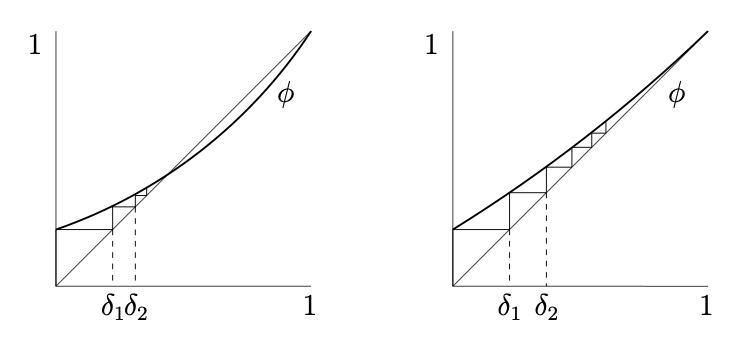
\includegraphics[scale = 0.4]{aaaa}
            \end{center}
            
            
            Assume $p_0 = G_1(0) > 0 $ and by convexity
            \begin{itemize}
            	\item If $G'(1) = \expt(Y) > 1$, $\prob_e = \lim_{n \rightarrow \infty}\,G_n(0)<1$
            	\item If $G'(1) = \expt(Y) < 1$, $\prob_e = 1$
            	\item If $G'(1) = \expt(Y) = 1$ : If $G''(1) > 0$, same graph as for $G'(1) < 1$; If $G''(1) = 0$, $Var(y) = 0$, then the process is deterministic and $Z_n = 1$ $\forall n$. \textcolor{red}{啥意思??}
            \end{itemize}
            
            \begin{theorem}
            	Let $\mu = \expt(Y)$ and $\sigma^2 = Var(Y)$ where $Y$ is the reproduction law. Then $\eta$, the probability of extinction is the smallest non-negative root of $s = G_Y(s)$ and  
            	\[
            	\eta = 1\,,\,\,\text{if $\mu$ < 1 or [$\mu$ = 1 and $\sigma^2$ > 0]}
               	\]
               	\[
               	\eta < 1\,,\,\,\text{if $\mu > 1$}
               	\]
            \end{theorem}
            
            \begin{remark}
            	该定理符合猜测:每一个individual都要生产出足够多的后代($\mu > 1$)以保证population 延续(renew),即使得不一定灭绝。
            \end{remark}
            
            \textcolor{blue}{对于discrete M.C的介绍到此为止。之后自学MCMC和HMM。}
            
            \bigskip
            
            \item \textbf{Exponential Distribution and Poisson Process}
            
            \smallskip
            
            \begin{definition}
            	(Exponential distribution) $\mathcal{X} \sim Exp(\lambda)$ The pdf of a expo. distributed r.v is 
            	\[
            	f(x) = \lambda e^{-\lambda x}\implies \expt(X) = \frac{1}{\lambda},\,\,Var(X) = \frac{2}{\lambda^2}
            	\]
            	\[
            	F(X) = \prob(X \leq x) = \int^x_0 \lambda e^{-\lambda x} dx = 1 - e^{-\lambda x}
            	\]
            	for $x$ defined only on $[0,\infty)$. Its MGF is 
            	\[
            	\phi(t) = \frac{\lambda}{\lambda - t} 
            	\]
            	for $t < \lambda$ and infinity for $t \geq \lambda$, since the integral goes to infinity. 
            \end{definition}
            
            \smallskip
            
            \begin{proposition}
            	(Memoryless property) In short 
            	\[
            	\prob(X > s+t)\,|\,X > s) = \prob(X>t)
            	\]
            	具体证明解释查看302 note。该性质说明已知目前正在进行,这对下一个时刻是否还会进行没有任何影响。            \end{proposition}
      
                 一个运算的例子
            	\[
            	  \prob(X>5\,|\,X>2) = \prob(X>3) = e^{-3 \lambda}
            	\]
            	
            	
            	
            	\begin{remark}
            		We can associate the exponential distribution as a measure of lifetime, from which we can qualify a \textit{failure rate} as follows.
            		\end{remark}
            		
            		\medskip
            		
            		\underline{\textbf{Set up the failure rate}}
            		
            		\smallskip
            		
            		Let $X$ represent the life time of some object (physical life, battery life etc.). Then the probability that the object can still be alive for another $dt$ time given that it has already lived for t is 
            		\[
            		\prob(X \in [t, t+dt]\,|\,X>t) = \frac{\prob(X\in [t, t+dt])}{\prob(X>t)}
            		\]
            		\[
            		 = \frac{\scaleint{4ex}^{t+dt}_t \,f(u)du}{1 - F(t)} \,\,\,\overset{dt \rightarrow 0}{\longrightarrow}\,\,\, \frac{f(t) \,dt}{1 - F(t)} = r(t) \,dt
            		\]
            		where we define the \textit{failure rate function (or hazard rate function )} as 
            		\[
            		r(t) = \frac{f(t)}{1 - F(t)}
            		\]
            		
            		in this context where $X$ is exponentially distributed $r(t) = \lambda$. So the failure rate function for an exponential r,v is constant which \hilight{does not depend on time.} This is another version of the non-memory property. We can prove that the exponential r.v is the only real continuous memoryless r.v. \textcolor{blue}{Feb.14th note. For discrete cases, the geometric distribution also has memoryless property.}
            		
            		\medskip
            		
            		\underline{\textbf{Min. of two exponential r.v}}
            	    
            	    \smallskip
            	    
            	    Let $X_1 \sim Expo(\lambda_1)$ and $X_2 \sim Expo(\lambda_2)$. We define a new r,v $X$ which is $X  = Min.(X_1, X_2)$. We are interested in the prob. distribution of $X$ so it is neat here to find the prob. of $X > x$, this is 
            	    \[
            	     \prob(X > x) = 1 - F_X(x)=  \prob(X_1 > x, X_2>x) 
            	    \]
            	    \[
            	    \underbrace{=}_{independent} \prob(X_1 > x) \prob(X_2 > x) = e^{-\lambda_1 x}e^{-\lambda_2 x}
            	    \]
            		\[
            		 = e^{-(\lambda_1 + \lambda_2)x} 
            		\]
            	    This means, the new r.v $X$ is also a exponetially distributed r.v with $\lambda = \lambda_1 + \lambda_2$. Then we can generalize this to the case of $n$ expo. r.v which is 
            	    \begin{proposition}
            	    	Let $X_1, X_2, ..., X_n$ are $n$ independently r.v that follows $X_i \sim Exp(\lambda_i)$, $i \in [1,n]$. Then 
            	    	\[
            	    	X = \min(X_1, X_2, ..., X_n) \sim Exp(\sum^n_{i = 1}\,\lambda_i)
            	    	\]
            	    \end{proposition}
            	    
                   \underline{例}:现在有三个顾客,其中两个正在前台被服务。假设每个顾客的服务时间为随即变量且均服从指数分布$Exp(\lambda)$。问:预计三个顾客都完成服务离开的时间是多长? 
                   
                   \smallskip
                   
                   \underline{解}: Time until the 1st customer leave is a r.v $X = min(X_1, X_2) \sim Exp(2\lambda)$ and $\mathbb{E}(X) = 1/2\lambda$. The clock then restart with the second customer fill the position and again the r.v is $X$. Finally the sole customer left and the time as a r.v following $X' \sim Exp(\lambda)$. So the expected time is $1/2\lambda + 1/2\lambda + 1/\lambda$. 
                   
                   \smallskip
                   
                   \begin{proposition}
                   	If $X_1$ and $X_2$ are independent and follows $X_i \sim Exp(\lambda_i)$. Then 
                   	\[
                   	\prob(X_1 < X_2) = \frac{\lambda_1}{\lambda_1 + \lambda_2}
                   	\]
                   \end{proposition}
                   
                   \begin{proof}
                   	\[
                   	\prob(X_1 < X_2) = \int\int_{x_1 < x_2} f_{X_1}(x_1)f_{X_2}(x_2) dx_1 dx_2
                   	\]
                   	\[
                   	 = \int_0^{\infty}\lambda_2 e^{-\lambda x}\,dx_2 \int^{x_2}_{0} \underbrace{\lambda_1 e^{-\lambda_1 x}dx_1}_{=\prob(X_1 \leq x_2) = 1 - e^{-\lambda_1x_2}}
                   	\]
                   	\[
                   	 = \int_0^{\infty}\lambda_2 e^{-\lambda_2 x_2}\,dx_2 - \int^\infty_0\lambda_2 e^{-(\lambda_1 + \lambda_2)x_2}dx_2
                   	\]
                   	 \[
                   	  = 1 - \frac{\lambda_2}{\lambda_1 + \lambda_2} = \frac{\lambda_1}{\lambda_1 + \lambda_2}
                   	 \]
                   \end{proof}
                   
                   \begin{proposition}
                   	Let $\mathcal{Z} = \sum^n_{i = 1} X_i$ where X and Y are expo. distributed r.v with parameter $\lambda_i$. Then the probability density function is 
                   	\[
                   	f_{\mathcal{Z}} = \sum^n_{i = 1} [\prod_{j \neq i}\,       \frac{\lambda_j}{\lambda_j - \lambda_i}] \cdot \lambda_i \cdot e^{-\lambda_i t}
                   	\]
                   	then if we know all $X_i$s are i.i.d with same $\lambda$, then 
                   	\[
                   \mathcal{Z} = 	\sum_{i=1}^n\,X_i \sim \Gamma(n, \lambda)
                   	\]
                   	with density function 
                   	\[
                   	f(t) = \lambda e^{- \lambda t} \frac{(\lambda t)^{n-1}}{(n-1)!}\,\,\,\,\,\,\,\mathbb{E} (\mathcal{Z}) = \frac{n}{\lambda}\,\,\,\,\, Var(Z) = \frac{n}{\lambda^2}
                   	\]
                   \end{proposition}
                   
                   \textcolor{blue}{Graph here needed to show the changes of parameter.}
                   
                   \bigskip
                   
                   \item \underline{\textbf{The Poisson Process}}
                   
                   \medskip
                   
                   Two ways to describe the process: 
                   \begin{itemize}
                   	\item To generate the process via exponentially distributed r.v. as "arrival time"
                   	\item Emphasizes on the properties of the process as counting process (i.e a stochastic process $\mathcal{N} (t)$ that represents the total number of events by time t).
                   \end{itemize}
                   
                   
                   
                   
                   
                   
                   
                   \begin{enumerate} 
                   \item\textbf{The first description}
                   
                   \smallskip
                   
                   A poisson process with rate $\lambda$ is a counting process where the time between 2 event is $Exp(\lambda)$. The time until $n$ event happens is 
                   \[
                   T = \sum^n_{i=1}\, X_i,\,\,\,X_i \sim Exp(\lambda)
                   \]
                   where all $X_i$ are $i.i.d$. The $\lambda$ here represent the rate of job completion (i.e the average job taks $1/\lambda$ time unit /job, so rate fo job completion is 1/1/$\lambda$ \textcolor{red}{Why?})
                   
                   \medskip
                   
                   Let the counting process to be $N$ and 
                   \[
                   N(t) = \text{\# of jobs completed by time t}, t\geq 0
                   \]
                   
                   \bigskip
                   
                   \begin{center}
                   	
                   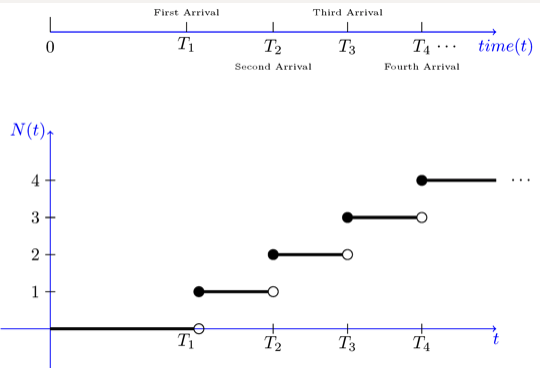
\includegraphics[scale = 0.36]{count}
                   
                   \end{center}
                   
                   We can conclude by intuition that 
                   \[
                   \mathbb{E}(N(t)) = \lambda t
                   \]
                   
                   \smallskip
                   
                   \underline{\textbf{PMF of N(t)}}
                   
                   \smallskip
                   
                   For $n \geq 1$, consider $\{N(t) \geq n\} \equiv \{\sum_{i = 1}^{n} X_i \leq t\}$. Both means $n$ jobs are completed by $t$. We have already derived the sum of exp. r.v follows Gamma distribution. Thus 
                   \[
                   \prob(N(t) \geq n) = \prob(\sum_{i = 1}^{n} X_i \leq t)
                   \]
                   \textcolor{red}{Proof made up here}. 
                   
                   \smallskip
                   
                   Finally we get 
                   \[
                   \prob(N(t) = m) = \frac{(\lambda t)^m e^{-\lambda t}}{m!}, m \geq 0
                   \]
                   which is the poisson distribution. So we conclude 
                   
                   \begin{theorem}
                   	If N(t) is a poisson process then 
                   	\[
                   	N(t) \sim Poisson(\lambda t)
                   	\]
                   	with mean $\lambda t$ and variance $\lambda t$. This matches our anticipation. 
                   \end{theorem}
                   
                   \underline{\textbf{Example}}
                   
                   \smallskip
                   
                   \begin{itemize}
                   	\item $\expt(S_4\,|\,N(1) = 2) = 1 + \expt (S_2) = 1 + 2/\lambda$
                   	\item $\expt(N(4) - N(2)\,|\,N(1) = 3) = \expt (N(4) - N(2)) = \expt(N(4-2)) = \expt(N(2)) = 2 \lambda$
                   \end{itemize}
                   对于以上问题可以直接画一个t的实轴分析。\textcolor{blue}{严谨证明在latex这个文件夹下的pdf里面}
                   \begin{proposition}
                   	\begin{itemize}
                   		\item \textit{Independent Increments:} If $(s_1, s_2)$ and $(t_1, t_2)$ are disjoint time interval, then $N(t_2) - N(t_1)$ and $N(s_2) - N(s_1)$ are independent r.vs. (This can be generalized to more than 2 intervals)
                   		\item \textit{Stationary Increments:} The difference between $N(s)$ and $N(s +t)$ is independent of $s$, in other words, same as $N(t)$. 
                   	\end{itemize}
                   \end{proposition}
                   
                   
                   \medskip
                   
                   \item \textbf{Second discrption:}
                   
                   \smallskip
                   
                   \begin{definition}
                   	(Poisson process) A counting process $\{N(t), t \geq 0\}$ is a poisson process of rate $\lambda$, if it satisfies the following axioms:
                   	\begin{itemize}
                   		\item N(0) = 0
                   		\item It has independent increment 
                   		\item $\prob(N(t + h) - N(t) = 1) = \lambda h + o(h)$
                   		\item $\prob (N(t + h)  - N(t) \geq 2) = o(h)$, or equivalently, $\prob(N(t + h) - N(t) = 0) = 1 - \lambda h + o(h)$  
                   	\end{itemize}
                   	where we define the $o(h)$ as the function $f$ which satisfy 
                   	\[
                   	\lim_{h \rightarrow 0} \frac{f(h)}{h} = 0 
                   	\]
                   \end{definition}
                   
                   \textcolor{red}{what is the function $o(h)$ means?}
                   
                   \smallskip
                   
                   The last axioms when we prove it, we can not treat $N(t)$ as a r.v following poisson distribution since that is what we are trying to show. We can only use theses axioms to prove it. 
                   
                   \begin{remark}
                   	A consequence of this 2nd definition is that 
                   	\[
                   	N(s+t) - N(s) \sim Poisson (\lambda t)
                   	\]
                   	This result is useful to show the equivalent of two definition of poisson process. \textcolor{red}{proof is in note March 2}.
                   \end{remark}
                   
                   \begin{theorem}
                   	We conclude from the above prove that two definition are equivalent that 
                   	\[
                   	\{N(t), t \geq 0\} \text{ is a Poisson process of rate $\lambda$ (by def. 2)}
                   	\]
                   	\[
                   	\Longleftrightarrow
                   	\]
                   	\[
                   	N(t) \text{is a counting process with iid inter arrival times $\sim Exp(\lambda) $(by def. 1)}
                   	\]
                   \end{theorem}
                   \textcolor{red}{Proof needed from March 2}
                   
                   \medskip
                   
                   \begin{theorem}
                   	(\textit{Superposition})\,\, Let $\{N_1(t), t \geq 0\}$ and $\{N_2(t), t \geq 0\}$ be two independent Poisson process, with rates $\lambda_1$ and $\lambda_2$. Then $N(t)$ is a poisson process of rate $\lambda_1 + \lambda_2$.
                   \end{theorem}   
                   
                   \textcolor{red}{Proof needed from note March 4.}                
                   \begin{proposition}
                   	(\textit{Poisson Timing}) Let $\{N(t), t \geq 0\}$ be a poisson process of rate $\lambda$ and that its events are independently labelled.: events are of either type 1 with prob. $p$ or type 2 with porb. $1 - p$. 
                   	
                   	\smallskip
                   	
                   	Let $N_1(t) = \#$ type 1 event by time t and $N_2(t)$ similarly. Then $N_1$ and $N_2$ are independent poisson process of rate $\lambda p$ and $\lambda (1 - p)$ respectively. 
                   \end{proposition}
                   \textcolor{red}{Proof as exercises, by showing the 5 axioms.}
                   \end{enumerate}
      
	\end{enumerate}

    \cleardoublepage
    
    \textbf{Questions}
    
    \begin{enumerate}
    	\item \sout{Does the initial prob. distribution have to be a row of the transition matrix?} 
    	\item \sout{For remark 3, we can keep multiplying the transition matrix because of time homo.?}
    	\item For the definition of $f_i$, we if we want to get back to $i$, there can be many way to achieve. So for proposition 3 the second property, how do we define the $f_i$?
    	
    \end{enumerate}

\end{changemargin}

\end{document}